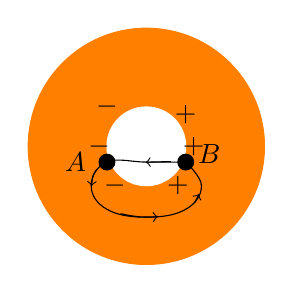
\begin{tikzpicture}
\draw  [fill, orange](0,0) circle (1.5);
\draw [fill, white]  (0,0) circle (0.5);
\node at (-0.5,0.5) {$-$};
\node at (-0.6,0) {$-$};
\node at (-0.4,-0.5) {$-$};
\node at (0.5,0.4) {+};
\node at (0.6,0) {+};
\node at (0.4,-0.5) {+};
\draw [fill] (-0.5,-0.2) node (v2) {} circle (0.1);
\draw  [fill] (0.5,-0.2) node (v1) {} circle (0.1);
\node at (-0.9,-0.2) {$A$};
\node at (0.8,-0.1) {$B$};
\draw  plot[smooth, tension=.7] coordinates {(v1) (0,-0.2) (v2) (-0.7,-0.5) (-0.5,-0.8) (0,-0.9) (0.5,-0.8) (0.7,-0.5) (0.5,-0.2)};
\draw [->] plot[smooth, tension=.7] coordinates {(-0.3281,-0.8552) (-0.0945,-0.8942) (0.1468,-0.8942)};
\draw  [->] plot[smooth, tension=.7] coordinates {(0.6139,-0.7151) (0.6684,-0.6061)};
\draw   [->]plot[smooth, tension=.7] coordinates {(0.3103,-0.1935) (-0.0089,-0.2013)};
\draw  [->] plot[smooth, tension=.7] coordinates {(-0.6317,-0.2947) (-0.6784,-0.3804) (-0.694,-0.5049)};
\end{tikzpicture}